\chapter{Konvertierung von GIS-Daten}
\label{converter-build}

\section{Idee}
Für die Konvertierung von GIS-Daten hatten wir die Idee, dies mit Hilfe eines Builds zu machen, d.h. ein Skript auf unserem Build-Server Jenkins (siehe Abschnitt \ref{build-server}) laufen zu lassen. Dadurch haben wir ein einfaches Web GUI für diese Aufgabe bekommen.

Der Converter-Build war zu Beginn ein sehr einfaches Hilfsmittel um Testdaten in Google Fusion Tables zu laden. Das Problem war, dass GFT von sich aus nur den Import von Google Spreadsheet, \gls{CSV}- und \gls{KML}-Dateien zu lässt, andere Formate sind nicht unterstützt. Viele frei verfügbare \gls{GIS}-Daten sind jedoch in anderen Formaten verfügbar, so dass eine Konvertierung zwangläufig notwendig ist. Zuerst haben wir jeweils den GeoConverter der HSR für diesen Zweck verwendet. Der Prozess ist allerdings etwas mühsam, da die konvenrtierte Datei dann jeweils noch manuell in GFT importiert werden muss.

Der Build ermöglicht es einfach und schnell beliebige Dateien zu konvertieren oder in GFT zu importieren.

\section{Implementation}
\subsection{Technischer Hintergrund}
Die Konvertierung basiert auf der Open Source Bibliothek GDAL/OGR.\footnote{\url{http://www.gdal.org/ogr}}.

Technisch gesehen ist der Converter-Build ein einfaches Ant-Skript welches das Kommandozeilen-Tool ogr2ogr\footnote{\url{http://www.gdal.org/ogr2ogr.html}} abstrahiert. Dieses Tool wird auf dem Server ausgeführt mit den entsprechend eingegebenen Parametern. 

\subsection{Features}
Da der Build auf ogr2ogr basiert, sind die Limitation durch dieses Tool gegeben. Es wird eine Vielzahl an \gls{GIS}-Formaten unterstützt\footnote{\url{http://www.gdal.org/ogr/ogr_formats.html}}. Speziell zu erwähnen ist dabei die Unterstützung für Google Fusion Tables, da wir damit die Möglichkeit bekommen haben, Daten direkt in GFT zu importieren\footnote{\url{http://www.gdal.org/ogr/drv_gft.html}}.

Für die anderen Formate wird jeweils das konvertierte File wieder zum Download angeboten.

\begin{figure}[!ht]
	\centering
	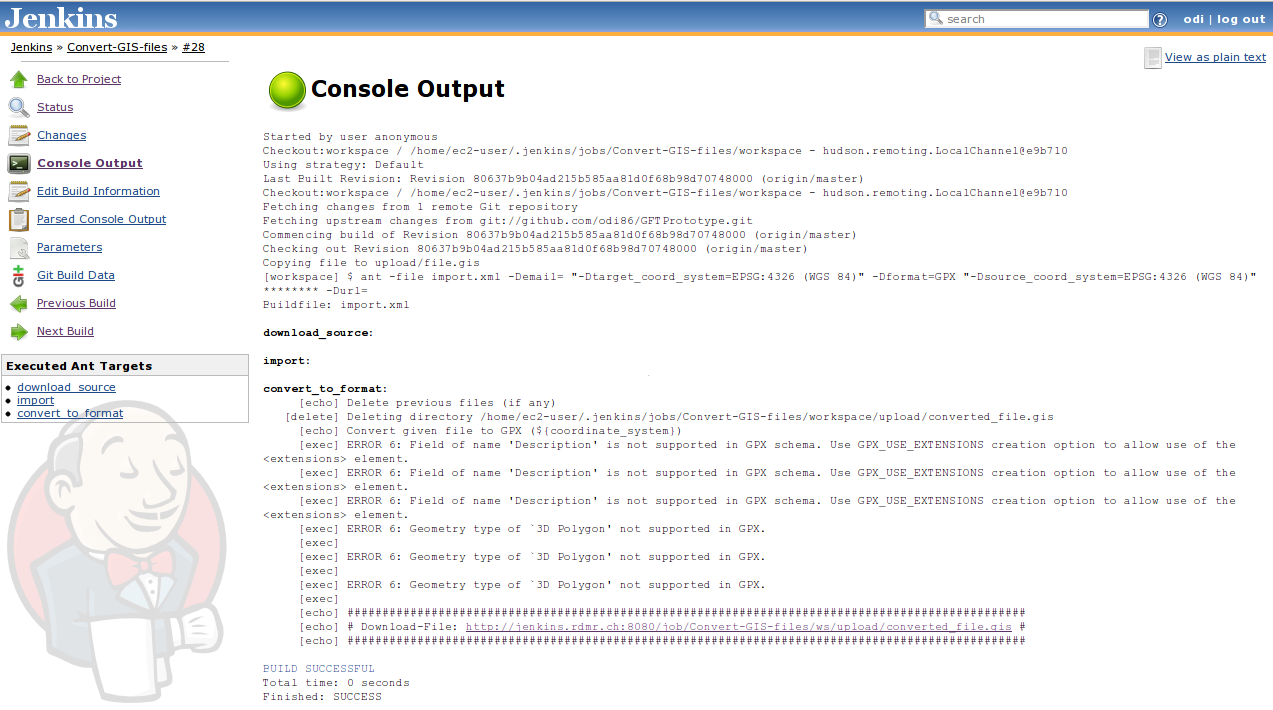
\includegraphics[width=\textwidth]{images/converter-build/converter-build-done}
	\caption{Wenn der Build abgeschlossen ist, lässt sich die konvertierte Datei herunterladen}
	\label{converter-build-done}
\end{figure}

Der Converter-Build nimmt sich die Input-Datei wahlweise von einem Upload oder von einer angegebenen URL. Weiter lässt sich das gewünschte Dateiformat und eine allfällige Koordinatenkonvertierung einstellen. Falls als Ausgabeformat \emph{GFT} gewählt wurde, muss man noch seine Angaben zu seinem Google-Konto angeben.

\begin{figure}[!ht]
	\centering
	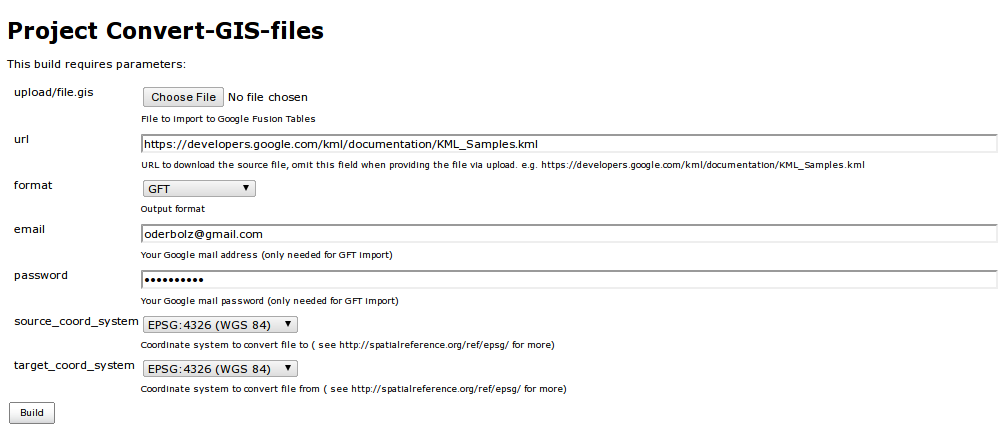
\includegraphics[width=\textwidth]{images/converter-build/converter-build-import}
	\caption{Optionen für den Converter-Build}
	\label{converter-build-import}
\end{figure}

\section{Installation}
Die Voraussetzungen für den Converter-Build sind zunächst eine Jenkins-Instanz, auf welcher das Plugin \emph{Parametetrized Build} installiert ist\footnote{\url{https://wiki.jenkins-ci.org/display/JENKINS/Parameterized+Build}}. Damit lassen sich an den Build via Web GUI Parameter übergeben. Grundsätzlich können damit generische Build-Jobs erstellt werden und dann je nachdem verschieden benutzt werden. 

Das Herzstück des Builds ist die GDAL/OGR Bibliothek welche sich aus dem Quellcode kompilieren lässt. Wichtig ist dabei, dass die Option \inlinecode{-{}-with-curl} angegeben wird, da ansonsten der GFT-Import nicht funktioniert.

\lstset{language=bash}
\begin{lstlisting}[caption=Kompilierung der GDAL/OGR Bibliothek mit cURL, label=converter-build-example]
$ ./configure --with-curl
$ make
# make install
\end{lstlisting}

Für die Koordinaten-Konvertierung muss zusätzlich noch die Bibliothek Proj.4\footnote{\url{http://trac.osgeo.org/proj/}} installiert werden.
